%#BIBTEX biber --bblencoding=utf8 -u -U --output_safechars main
\documentclass[uplatex, dvipdfmx]{article}
\usepackage{amsmath, amsthm, amssymb}
\usepackage{ascmac,here,txfonts,txfonts}
\usepackage[margin=2.5cm]{geometry}
\usepackage{tikz}
\usetikzlibrary{arrows}
\usepackage{graphicx}
\usepackage{algorithm}
\usepackage{algorithmic}
\usepackage{color}
\usepackage{xcolor}
\usepackage[subrefformat=parens]{subcaption}
\usepackage{hyperref}
\usepackage[backend=biber, style=numeric, sorting=none]{biblatex}
\usepackage[format=hang]{caption}
\usepackage[format=hang, subrefformat=parens]{subcaption}

\captionsetup{compatibility=false}

\addbibresource{./references.bib}

\setlength{\parindent}{0.3in}

\title{修士学位請求論文要旨\\
 Iterated Inversion System: An Efficient Algorithm to Visualize Kleinian Groups Based on Inversions }
\author{中村 建斗\\
先端数理科学研究科 先端メディアサイエンス専攻\\
}

\date{}

\pagestyle{plain}

\begin{document}

\maketitle
\pagestyle{plain}
\newpage

In this paper, we introduce a summary of each chapter of the master thesis.
The first chapter is an introduction.
Kleinian groups theory is one of the fields of mathematics.
It is advanced by mathematicians in the nineteenth century.
Felix Klein and Robert Fricke studied a certain category of M\"obius
transformation groups.
Henri Poincare named such groups \textit{Kleinian Groups}.

Kleinian groups are well suited to visualization and
experiment; Actually, Klein and his students also leave beautiful
visualized images of a Kleinian group without a computer.
After a computer appeared, various visualization and calculation are
performed by a computer.

Our final goals are to visualize all of the Kleinian groups in real time
by personal computers and to help us understand the Kleinian group theory
intuitively.
As the first step to the goals, we invent an algorithm called
\textit{Iterated Inversion System (IIS)}.
It visualizes not only three-dimensional Kleinian groups but also
four-dimensional Kleinian groups.

The second chapter is preparation. We introduce some mathematical terms.

\begin{figure}[htbp]
 \begin{minipage}[t]{0.3333\hsize}
  \center
  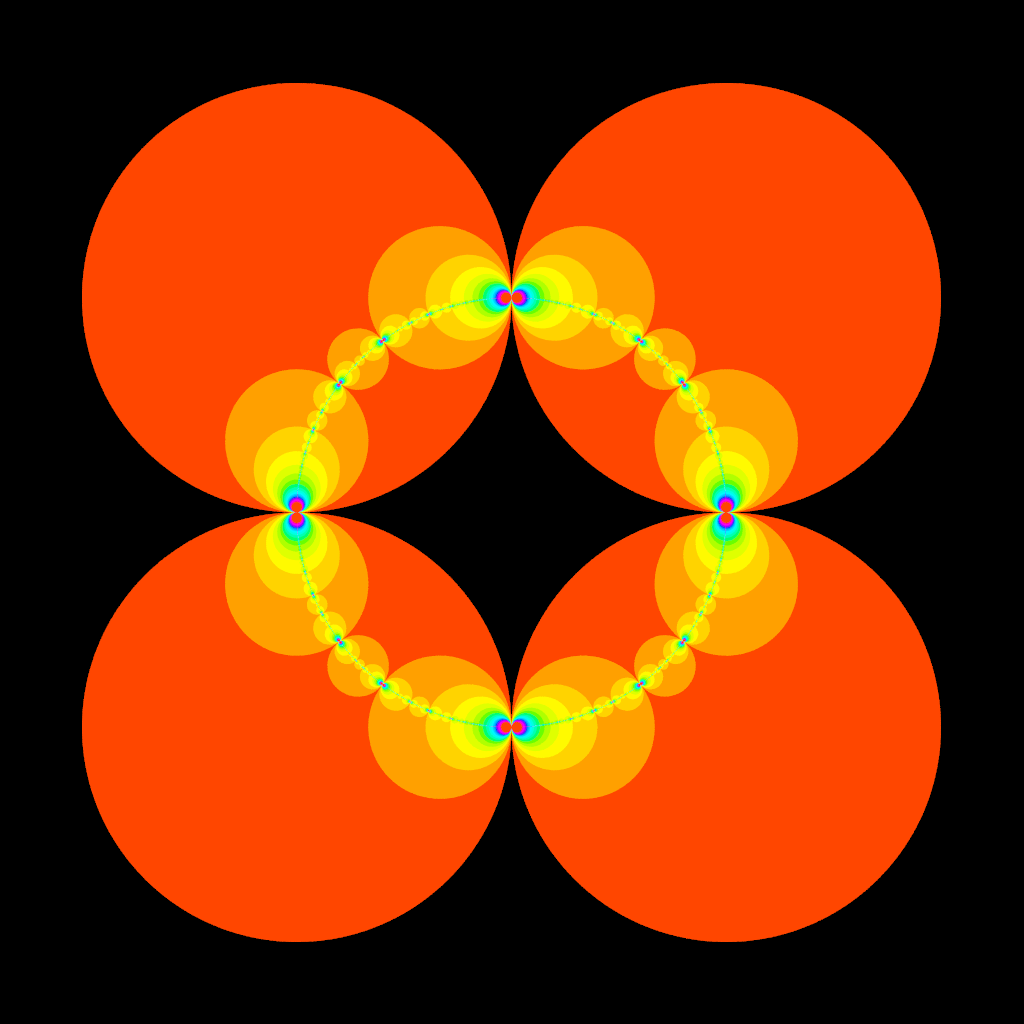
\includegraphics[height=1.35in, keepaspectratio]{../src/img/preparation/basic/circleOrbit.png}
  \caption{\textit{The orbit of the disks}}
  \label{fig:orbitCircles}
  \hspace*{\fill}
 \end{minipage}
 \begin{minipage}[t]{0.66666\hsize}
  \hspace*{\fill}
  \begin{minipage}[t]{0.3333\hsize}
   \center
   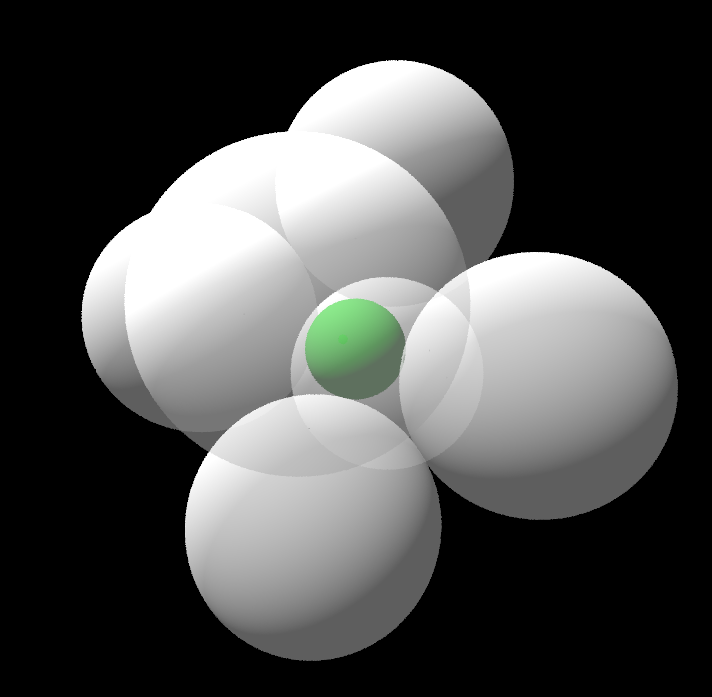
\includegraphics[height=1.35in, keepaspectratio]{../src/img/preparation/3dExtension/3dKissingGenerator.png}
   \subcaption{\textit{Generator}}
   \label{fig:3dGen}
  \end{minipage}
  \hspace*{\fill}
  \begin{minipage}[t]{0.3333\hsize}
   \center
   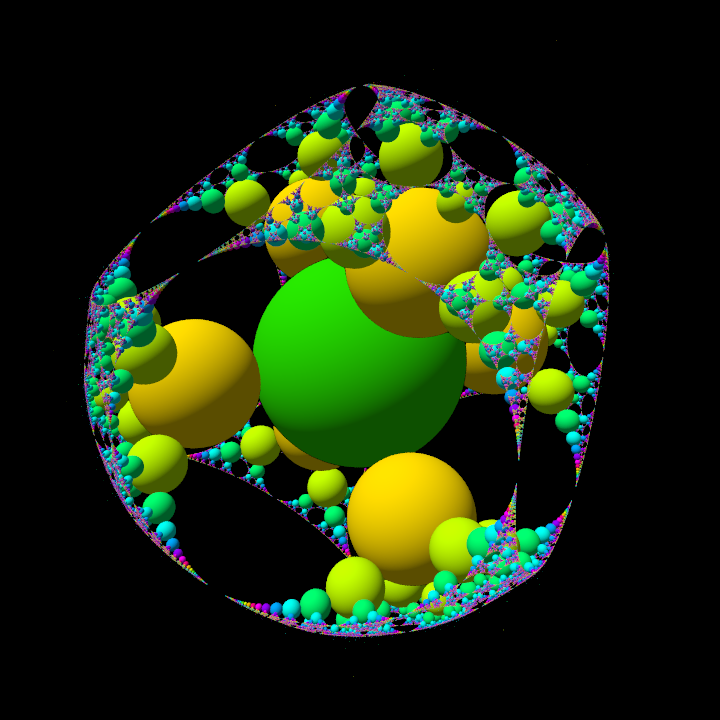
\includegraphics[height=1.35in, keepaspectratio]{../src/img/preparation/3dExtension/3dOrbit.png}
   \subcaption{\textit{The orbit of the sphere}}
   \label{fig:3dOrb}
  \hspace*{\fill}
  \end{minipage}
   \caption{\textit{The orbit of the sphere}}
  \label{fig:3d} 
 \end{minipage}
 \hspace*{\fill}
\end{figure}

\begin{figure}[htbp]
 \begin{minipage}[t]{0.5\hsize}
  \center
  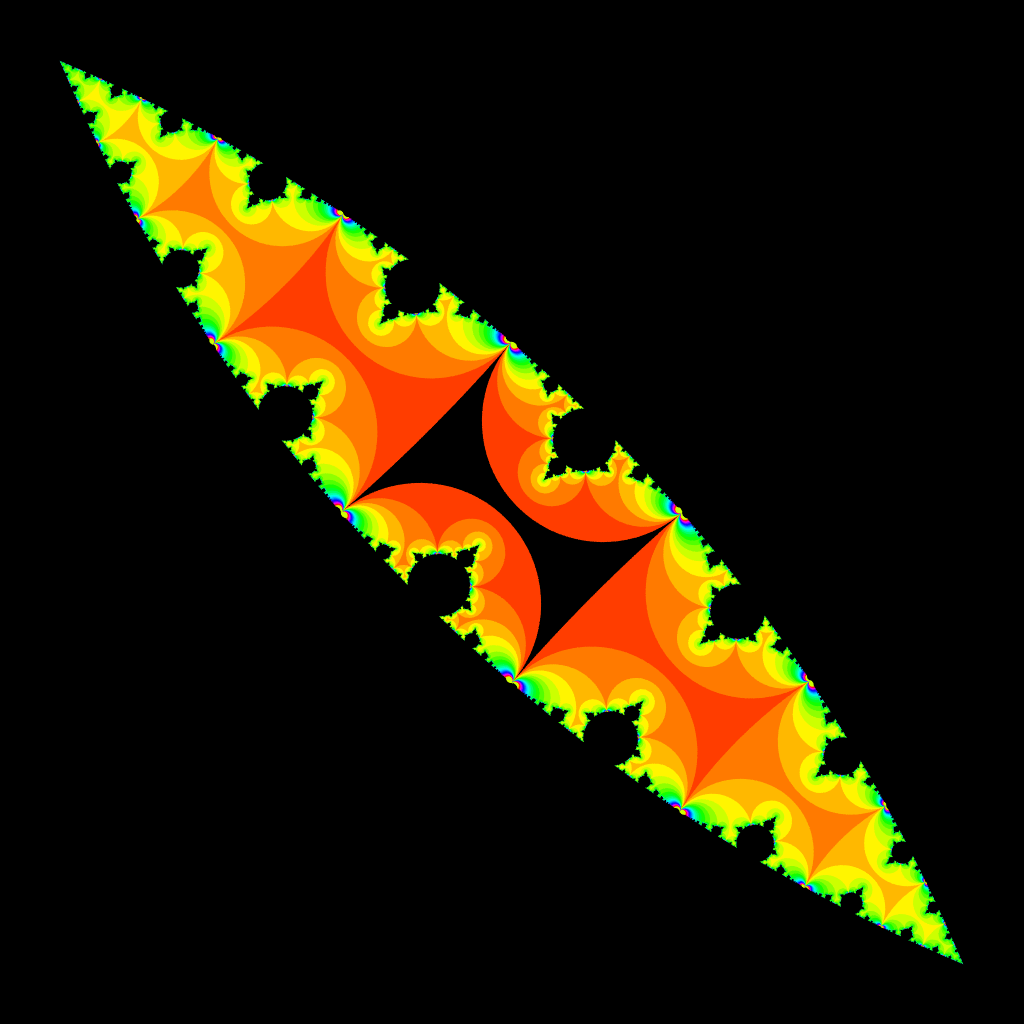
\includegraphics[height=1.35in, keepaspectratio]{../src/img/application/internal/schottky.png}
  \subcaption{\textit{}}
  \label{fig:schottkyAll}
  \hspace*{\fill}
 \end{minipage}
 \begin{minipage}[t]{0.5\hsize}
  \center
  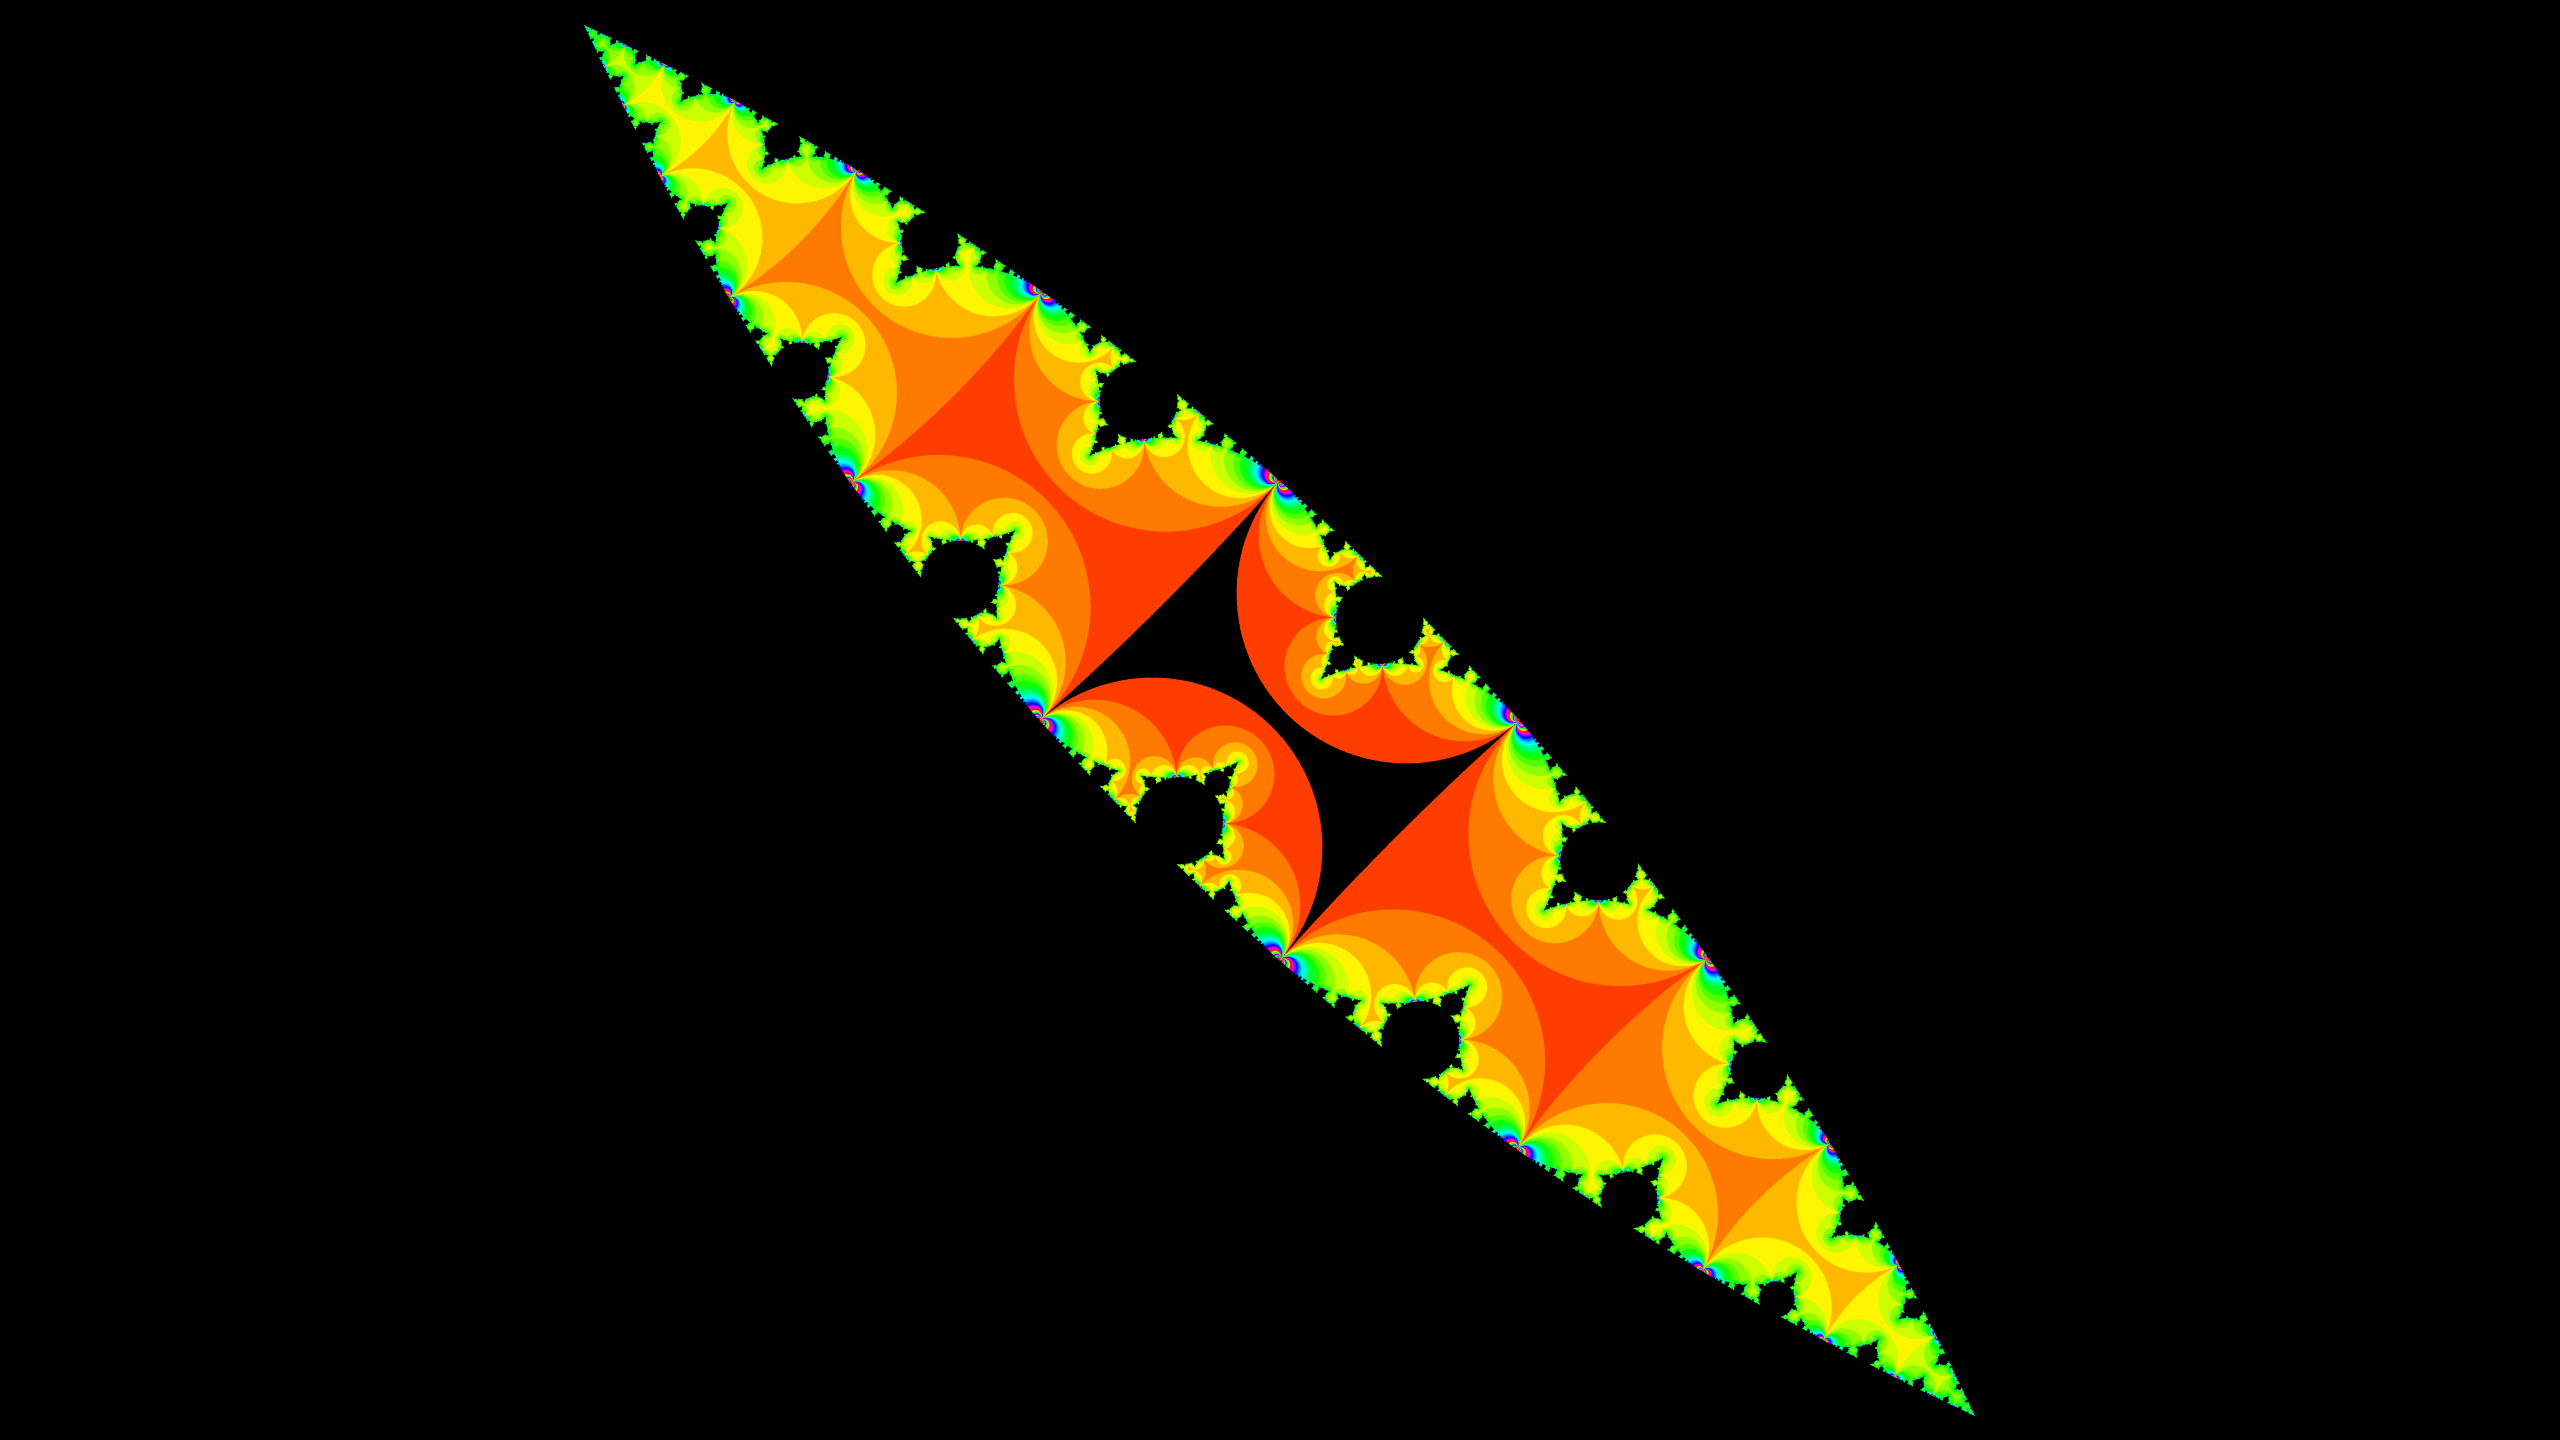
\includegraphics[height=1.35in, keepaspectratio]{../src/img/application/internal/schottkyEdge.png}
  \subcaption{\textit{}}
  \label{fig:schottkyEdge}
  \hspace*{\fill}
 \end{minipage}
 \caption{\textit{Edge of the circle inversion fractal}}
 \label{fig:schottkyDivide}
\end{figure}

\begin{figure}[htbp]
 \begin{minipage}[t]{0.5\hsize}
  \center
  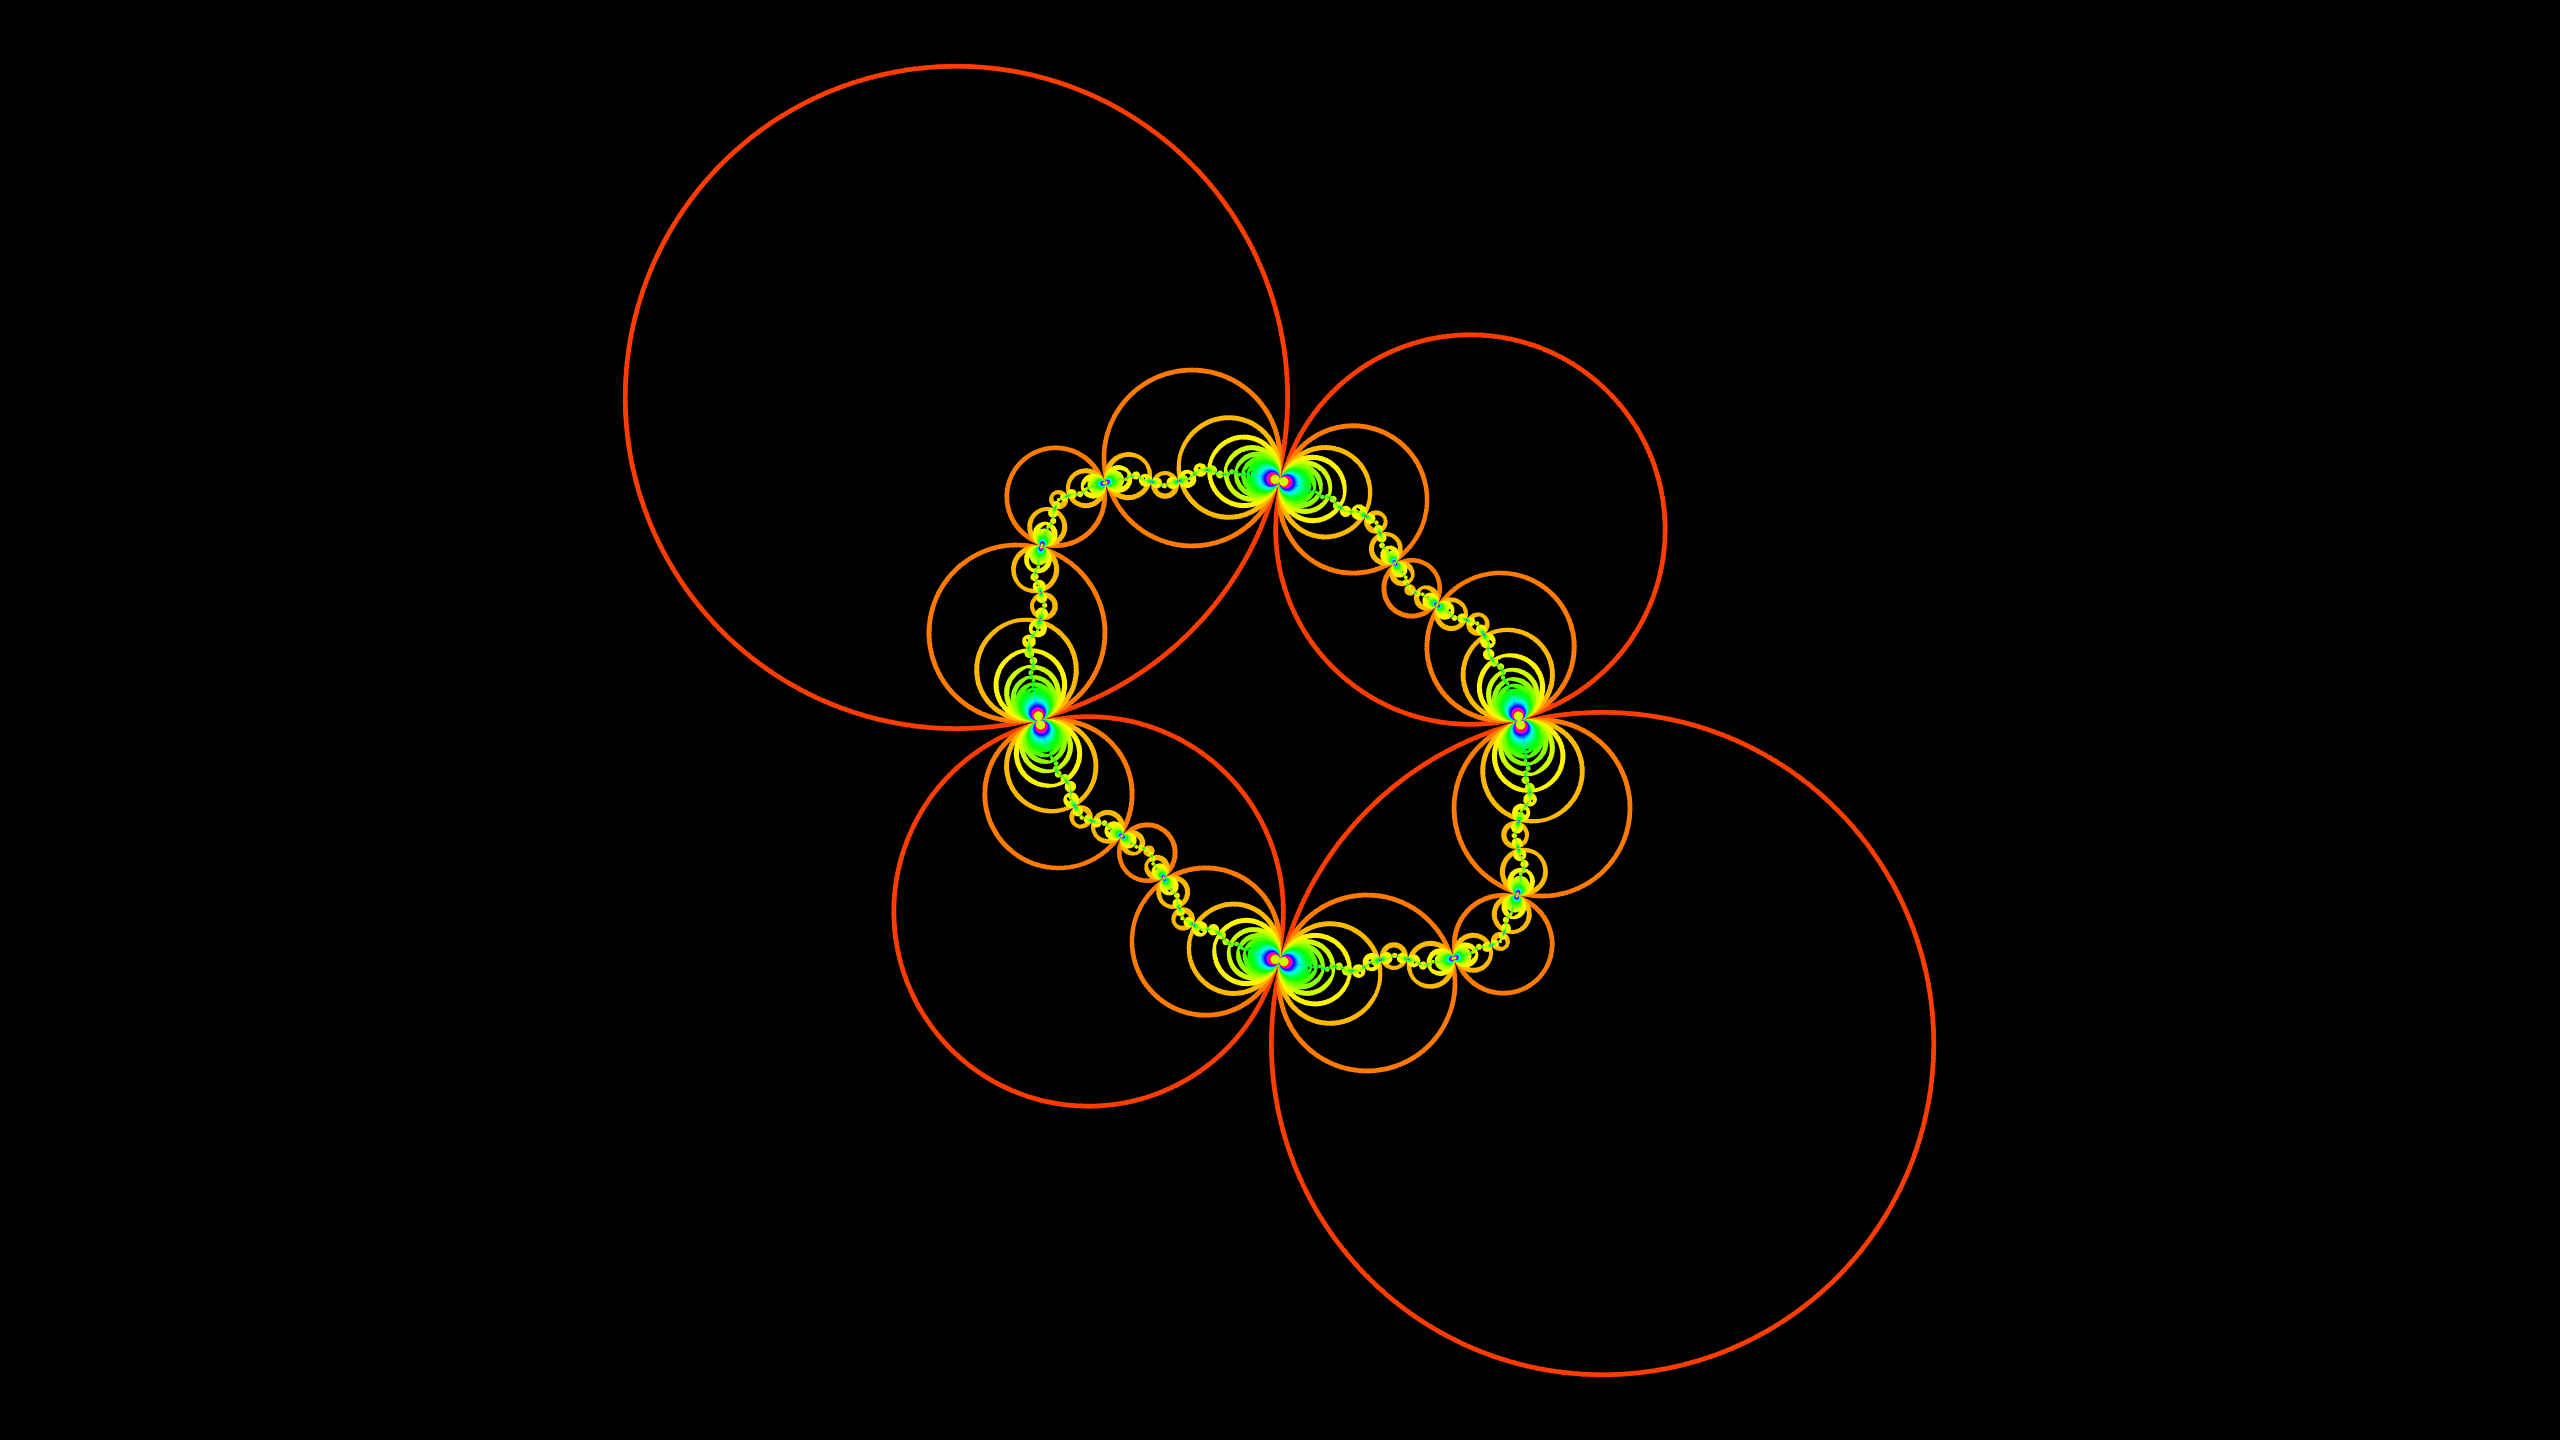
\includegraphics[height=1.35in, keepaspectratio]{../src/img/application/edge/circles.png}
  \subcaption{\textit{}}
  \label{}
  \hspace*{\fill}
 \end{minipage}
 \begin{minipage}[t]{0.5\hsize}
  \center
  \includegraphics[height=1.35in, keepaspectratio]{../src/img/application/edge/circleEdge.png}
  \subcaption{\textit{}}
  \label{}
  \hspace*{\fill}
 \end{minipage}
 \caption{\textit{Circle inversion fractal}}
 \label{fig:circleEdge}
\end{figure}

\begin{figure}[htbp]
 \begin{minipage}{0.5\hsize}
  \begin{minipage}{0.25\hsize}
   \center
   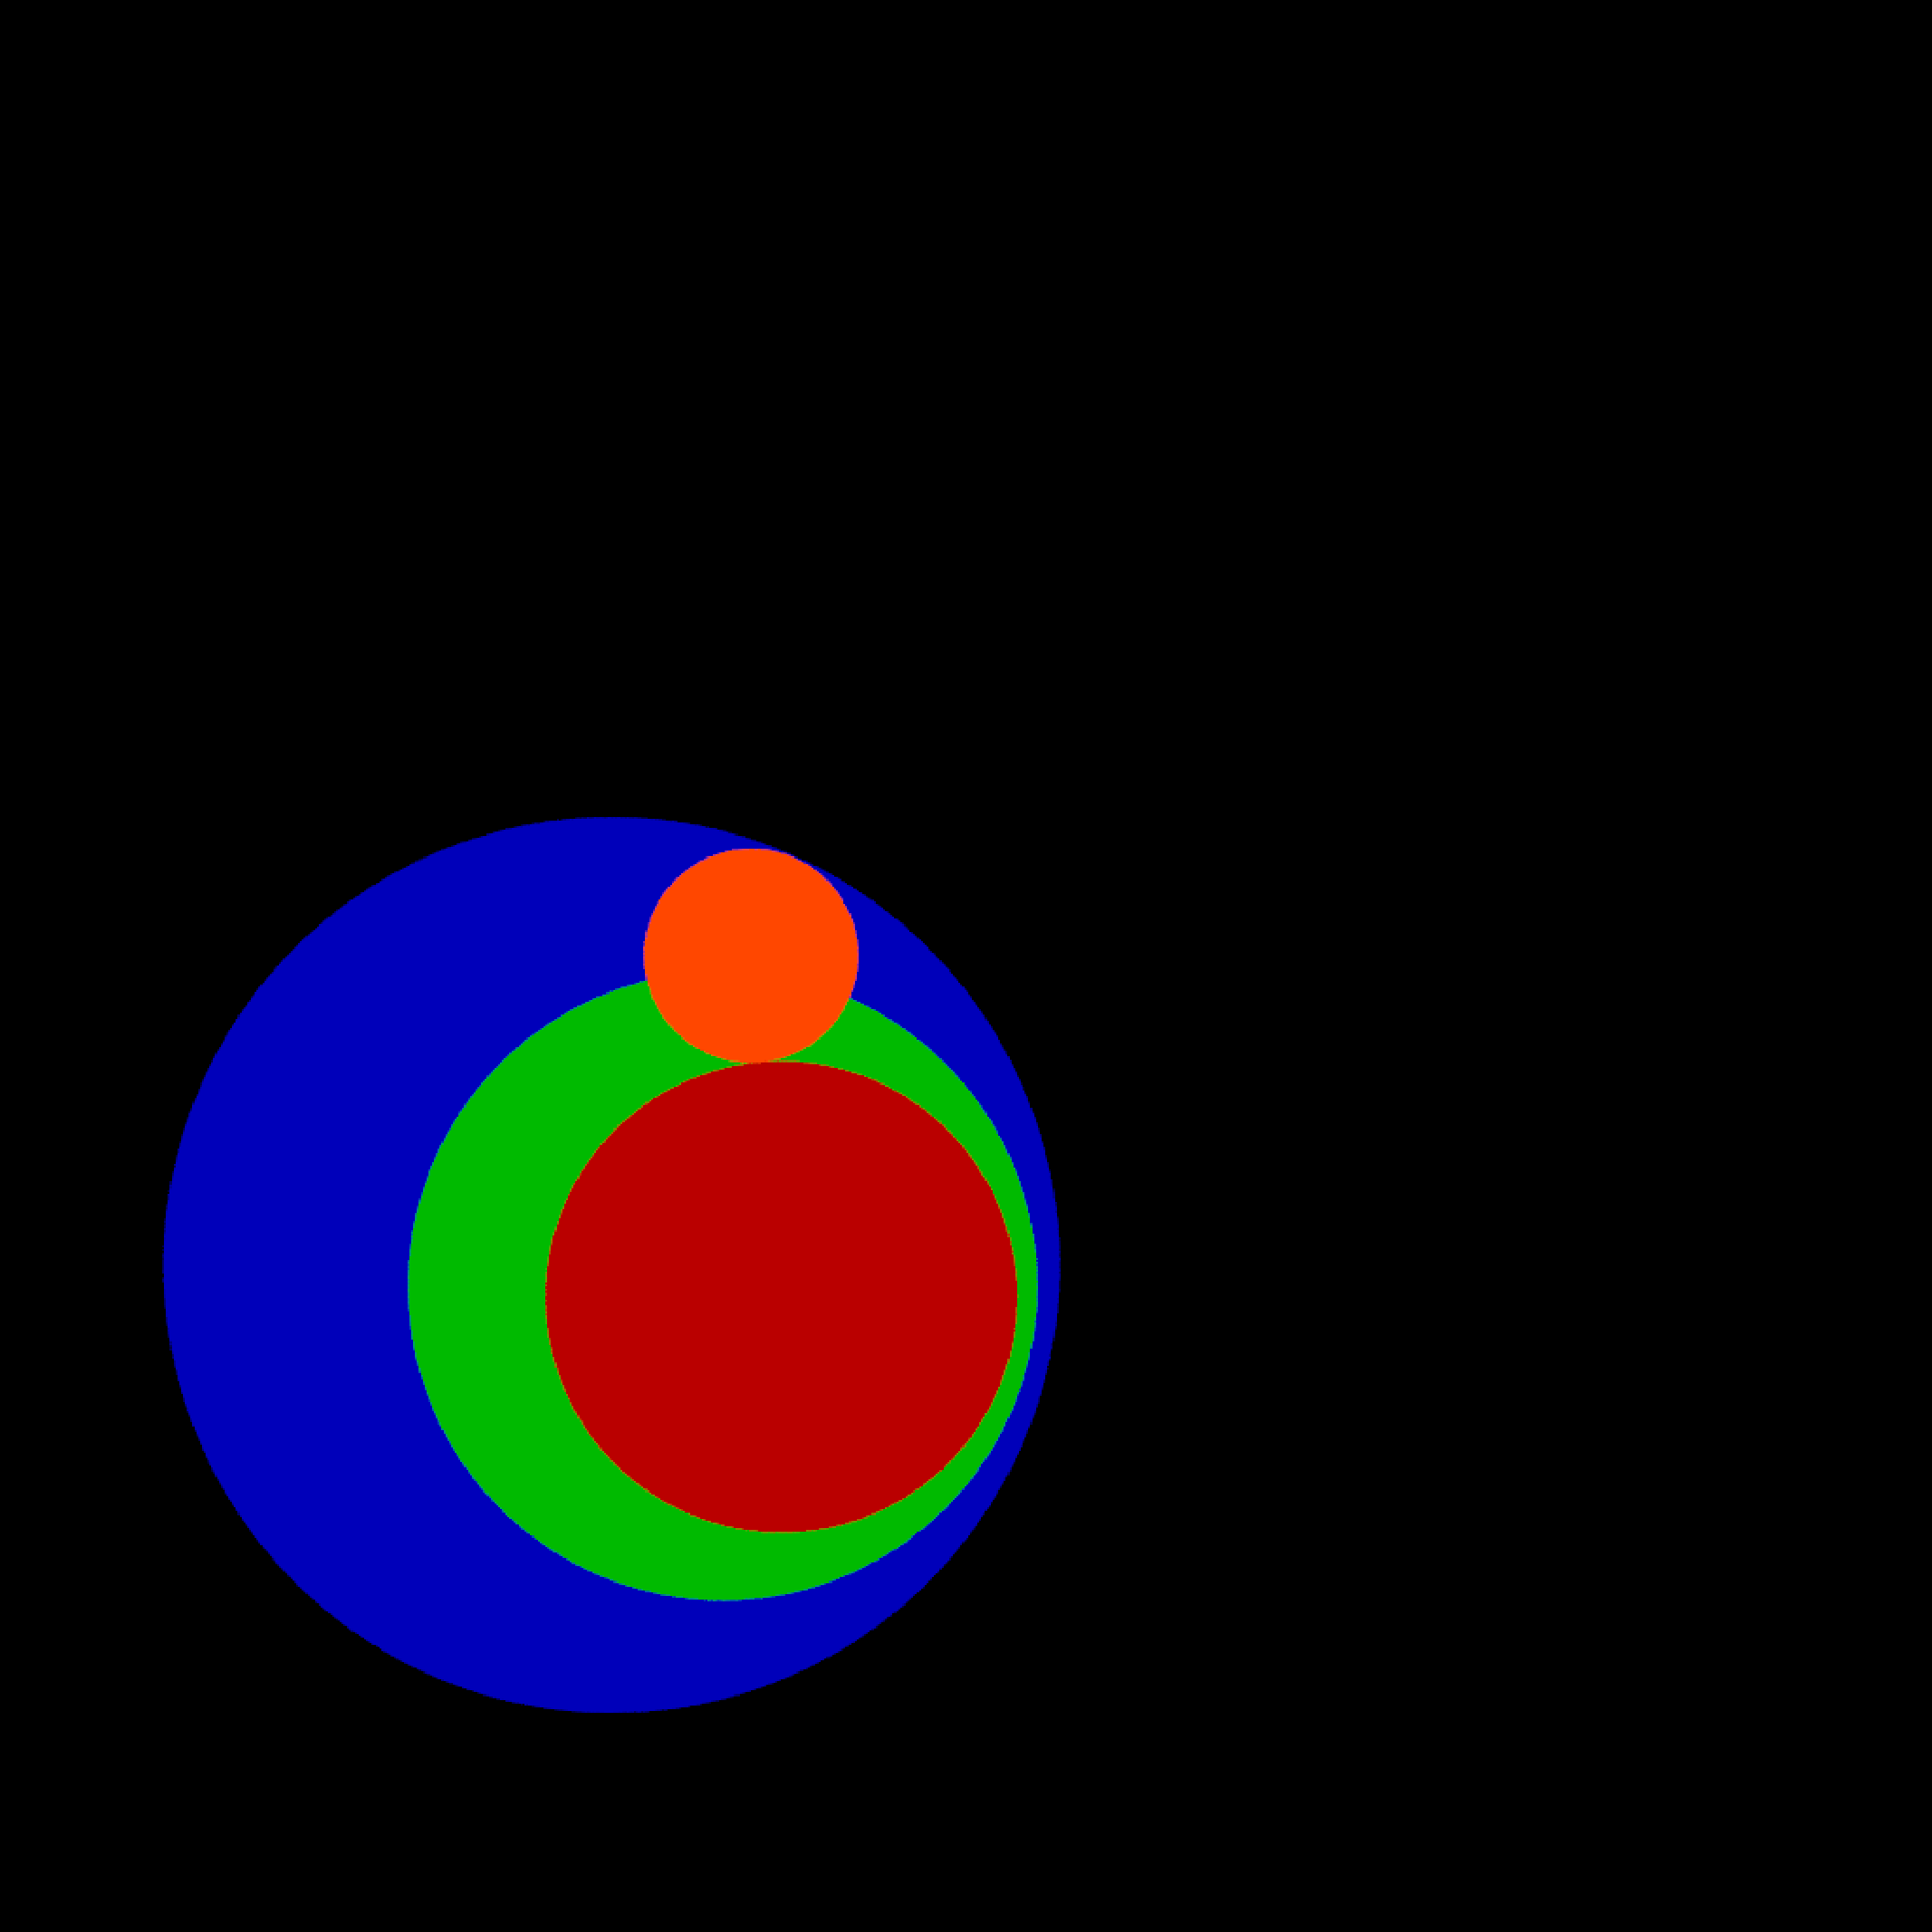
\includegraphics[ height=1.4in, keepaspectratio]{../src/img/application/2dGen/hyperbolicRect0.pdf}
   \subcaption{\textit{Generator}}
   \label{fig:hyperbolic2dGen}
  \end{minipage}
 \hspace*{\fill}
  \begin{minipage}{0.25\hsize}
   \center
   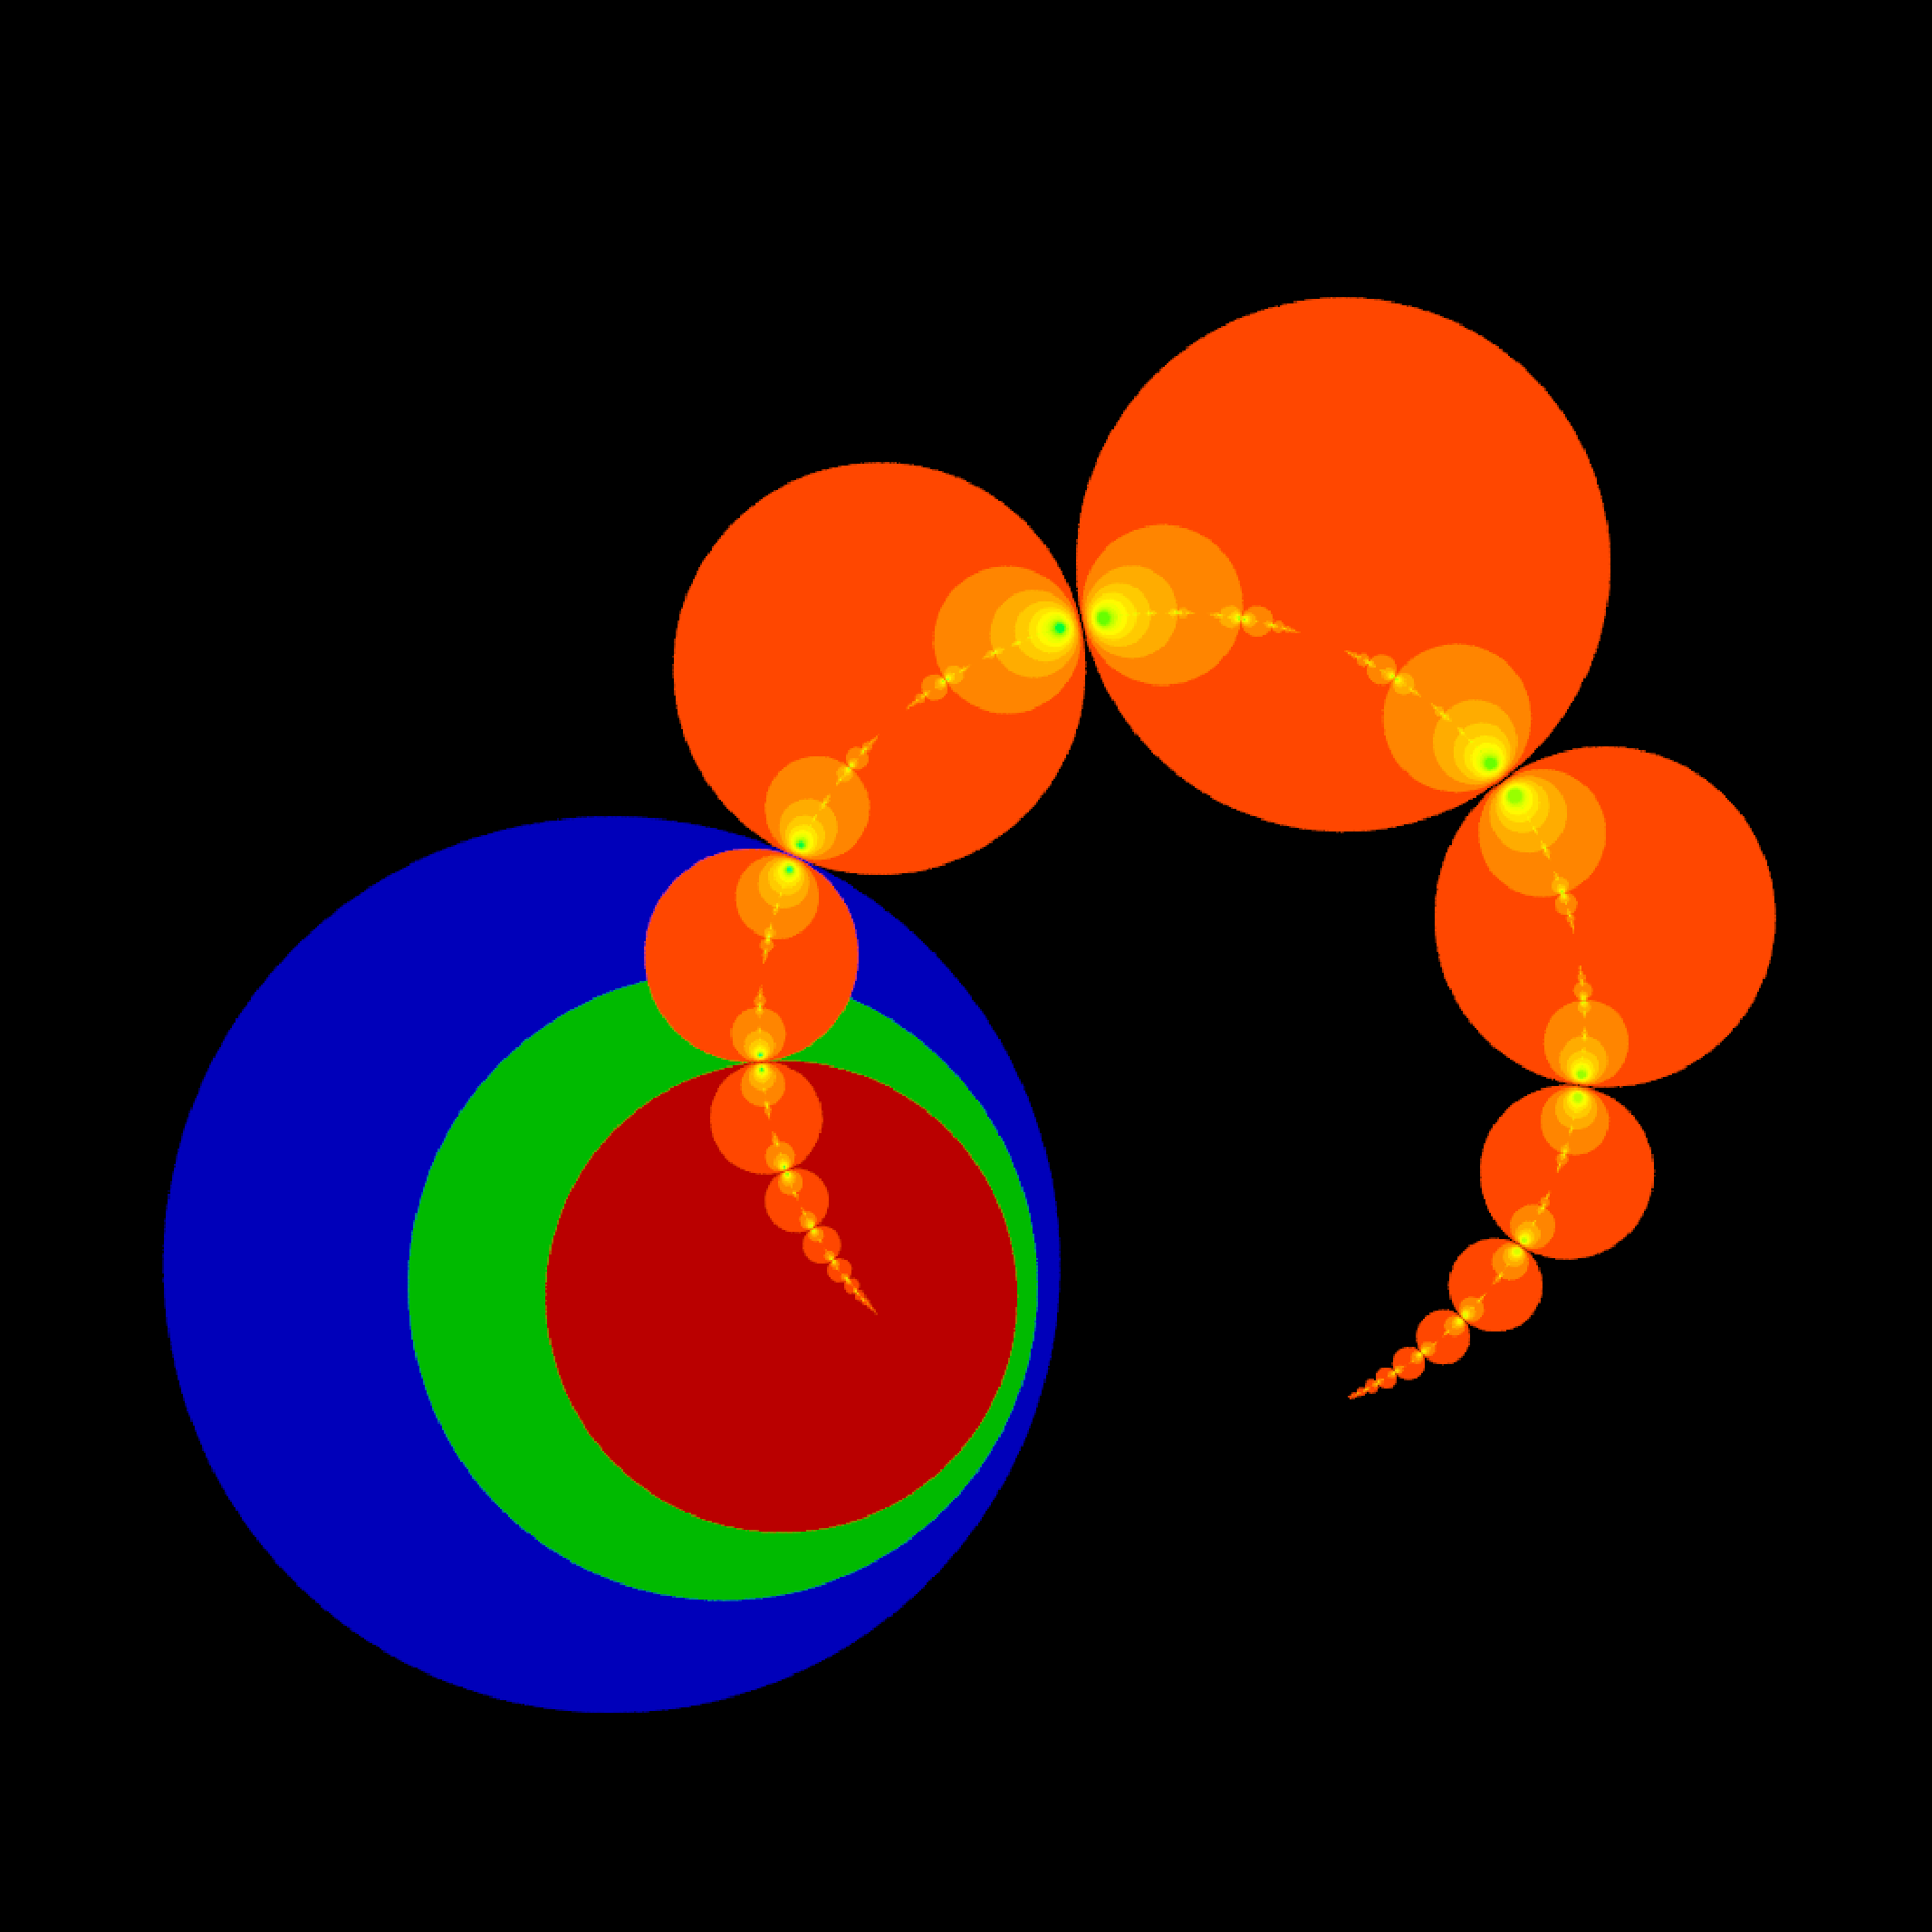
\includegraphics[ height=1.4in, keepaspectratio]{../src/img/application/2dGen/hyperbolicRect.pdf}
   \subcaption{\textit{Orbit}}
   \label{fig:hyperbolic2dOrb}
  \end{minipage}
 \hspace*{\fill}
  \caption{\textit{Hyperbolic generator and a Schottky disk}}
  \label{fig:hyperbolic2d}
 \end{minipage}
 \begin{minipage}[t]{0.5\hsize}
  \begin{minipage}{0.25\hsize}
   \center
   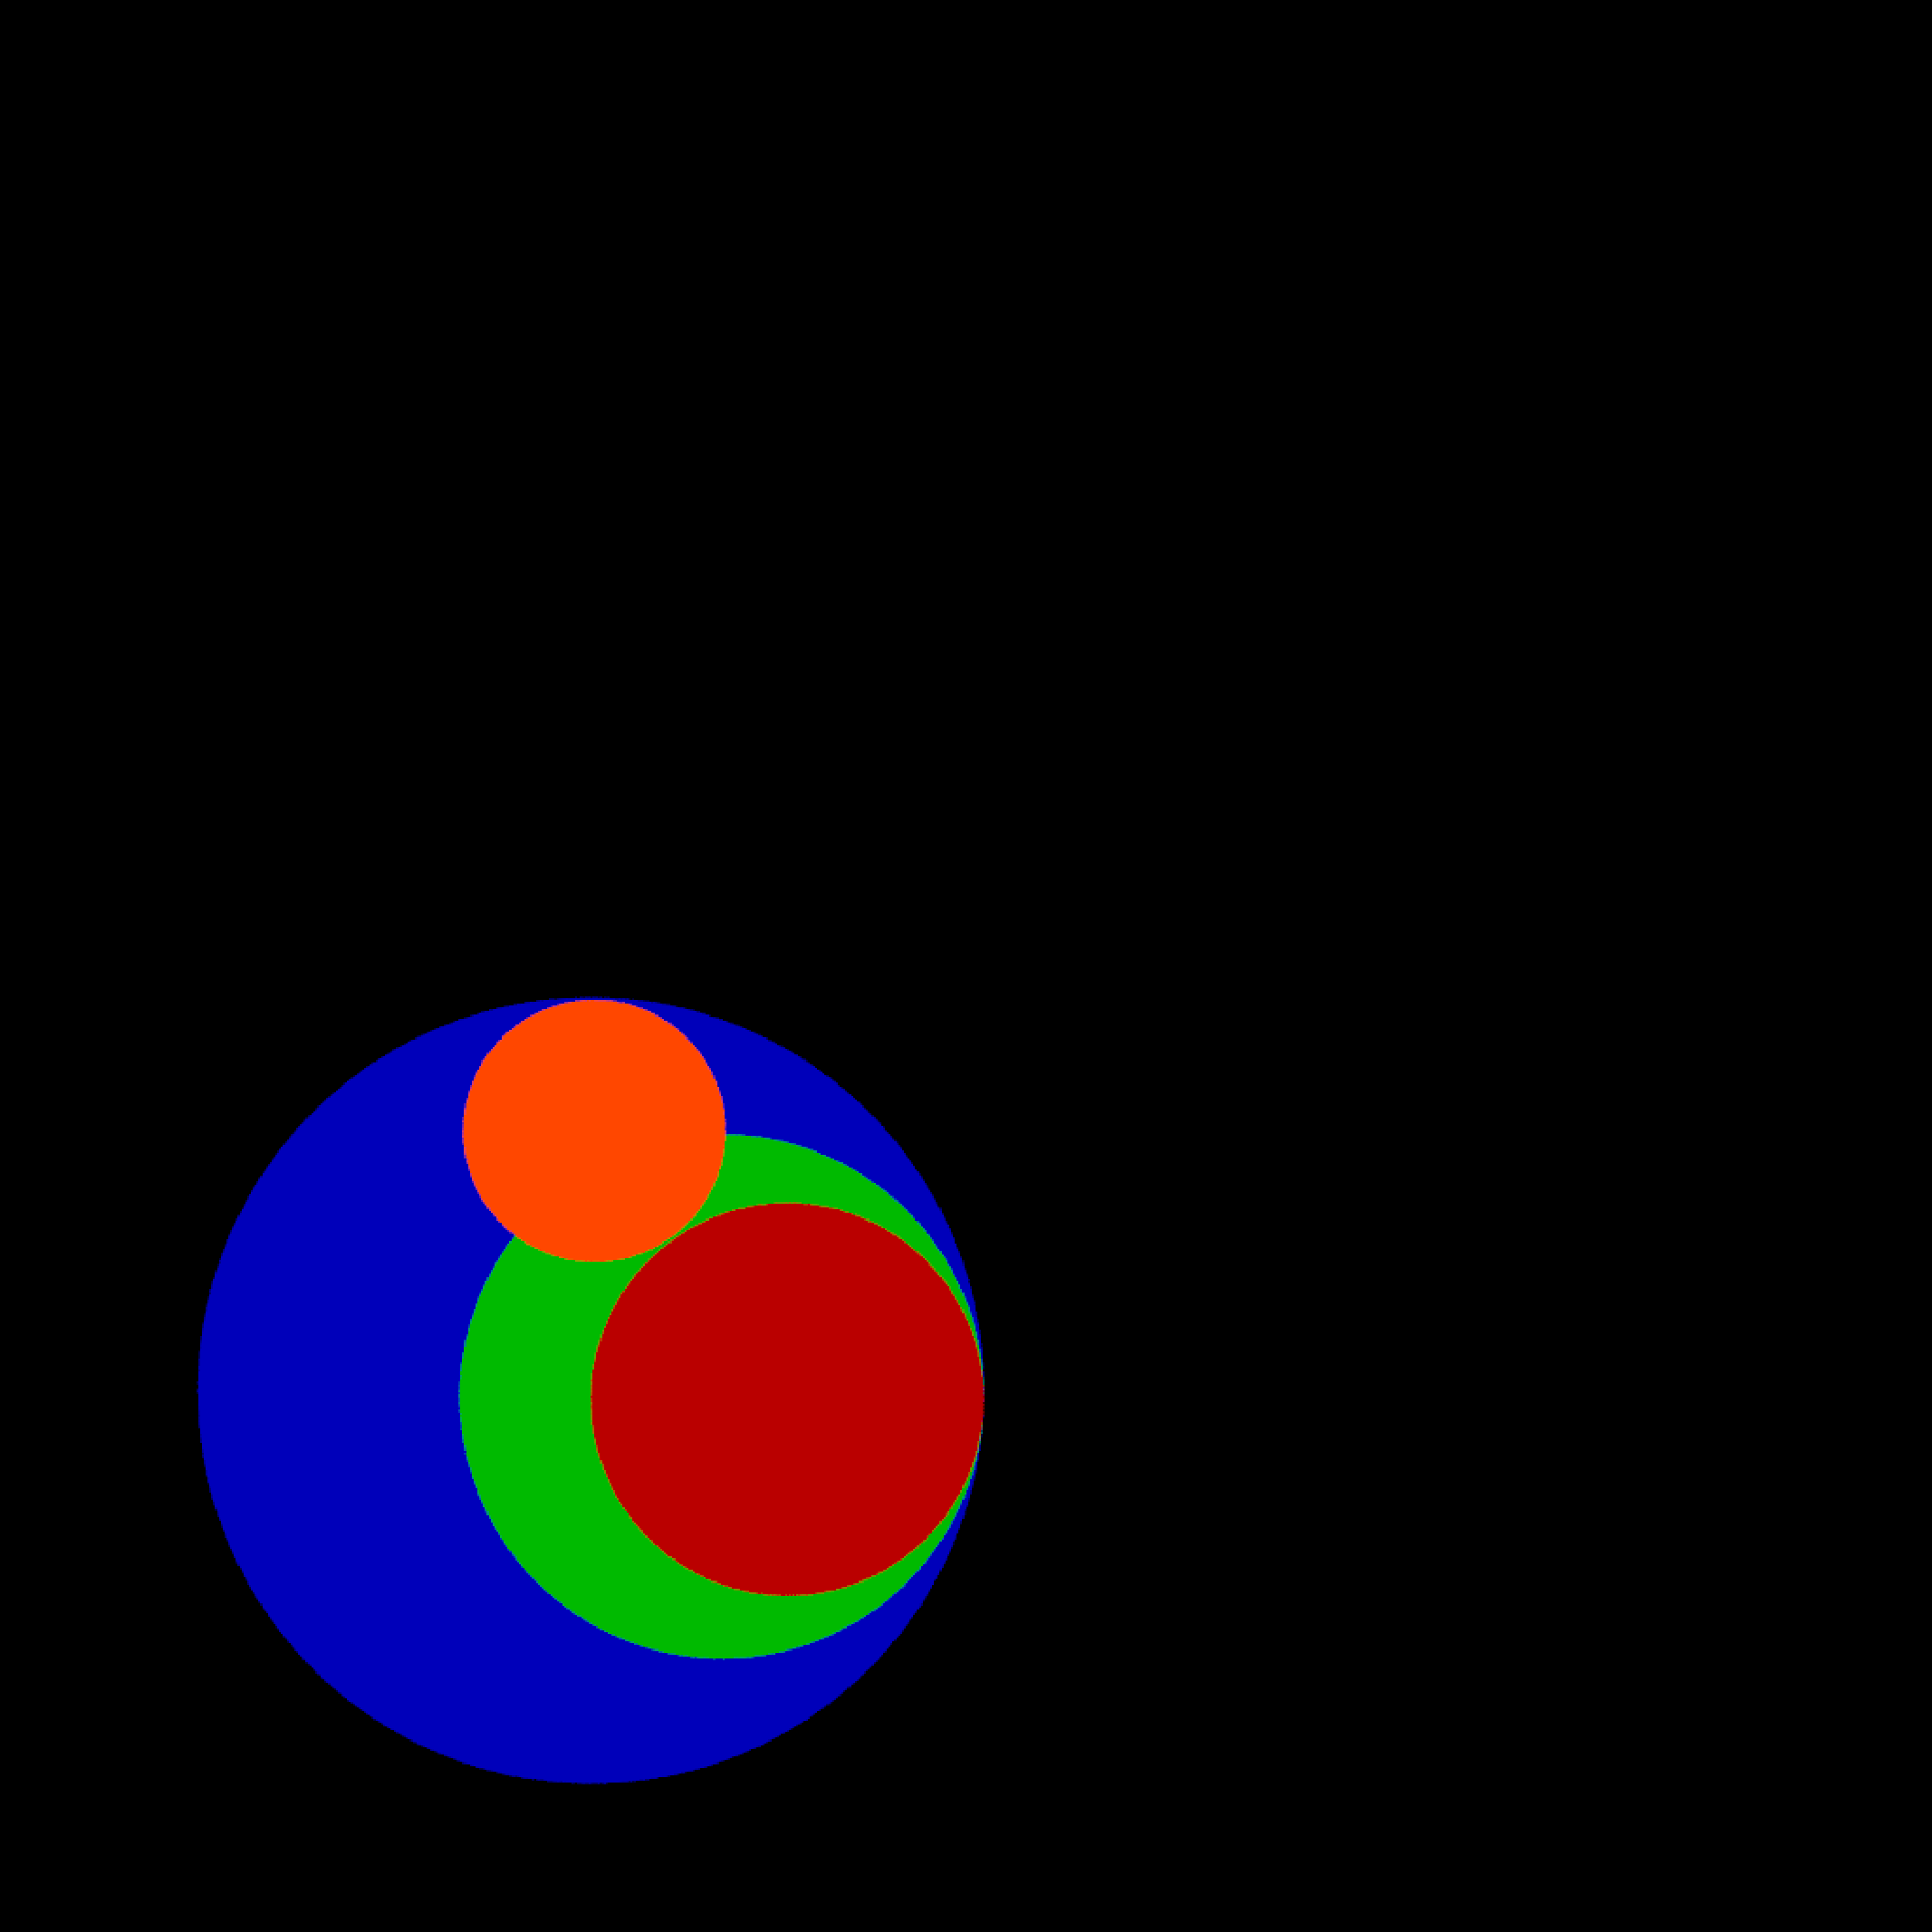
\includegraphics[ height=1.4in, keepaspectratio]{../src/img/application/2dGen/parabolicRect0.pdf}
   \subcaption{\textit{Generator}}
   \label{fig:parabolic2dGen}
  \end{minipage}
 \hspace*{\fill}
  \begin{minipage}{0.25\hsize}
   \center
   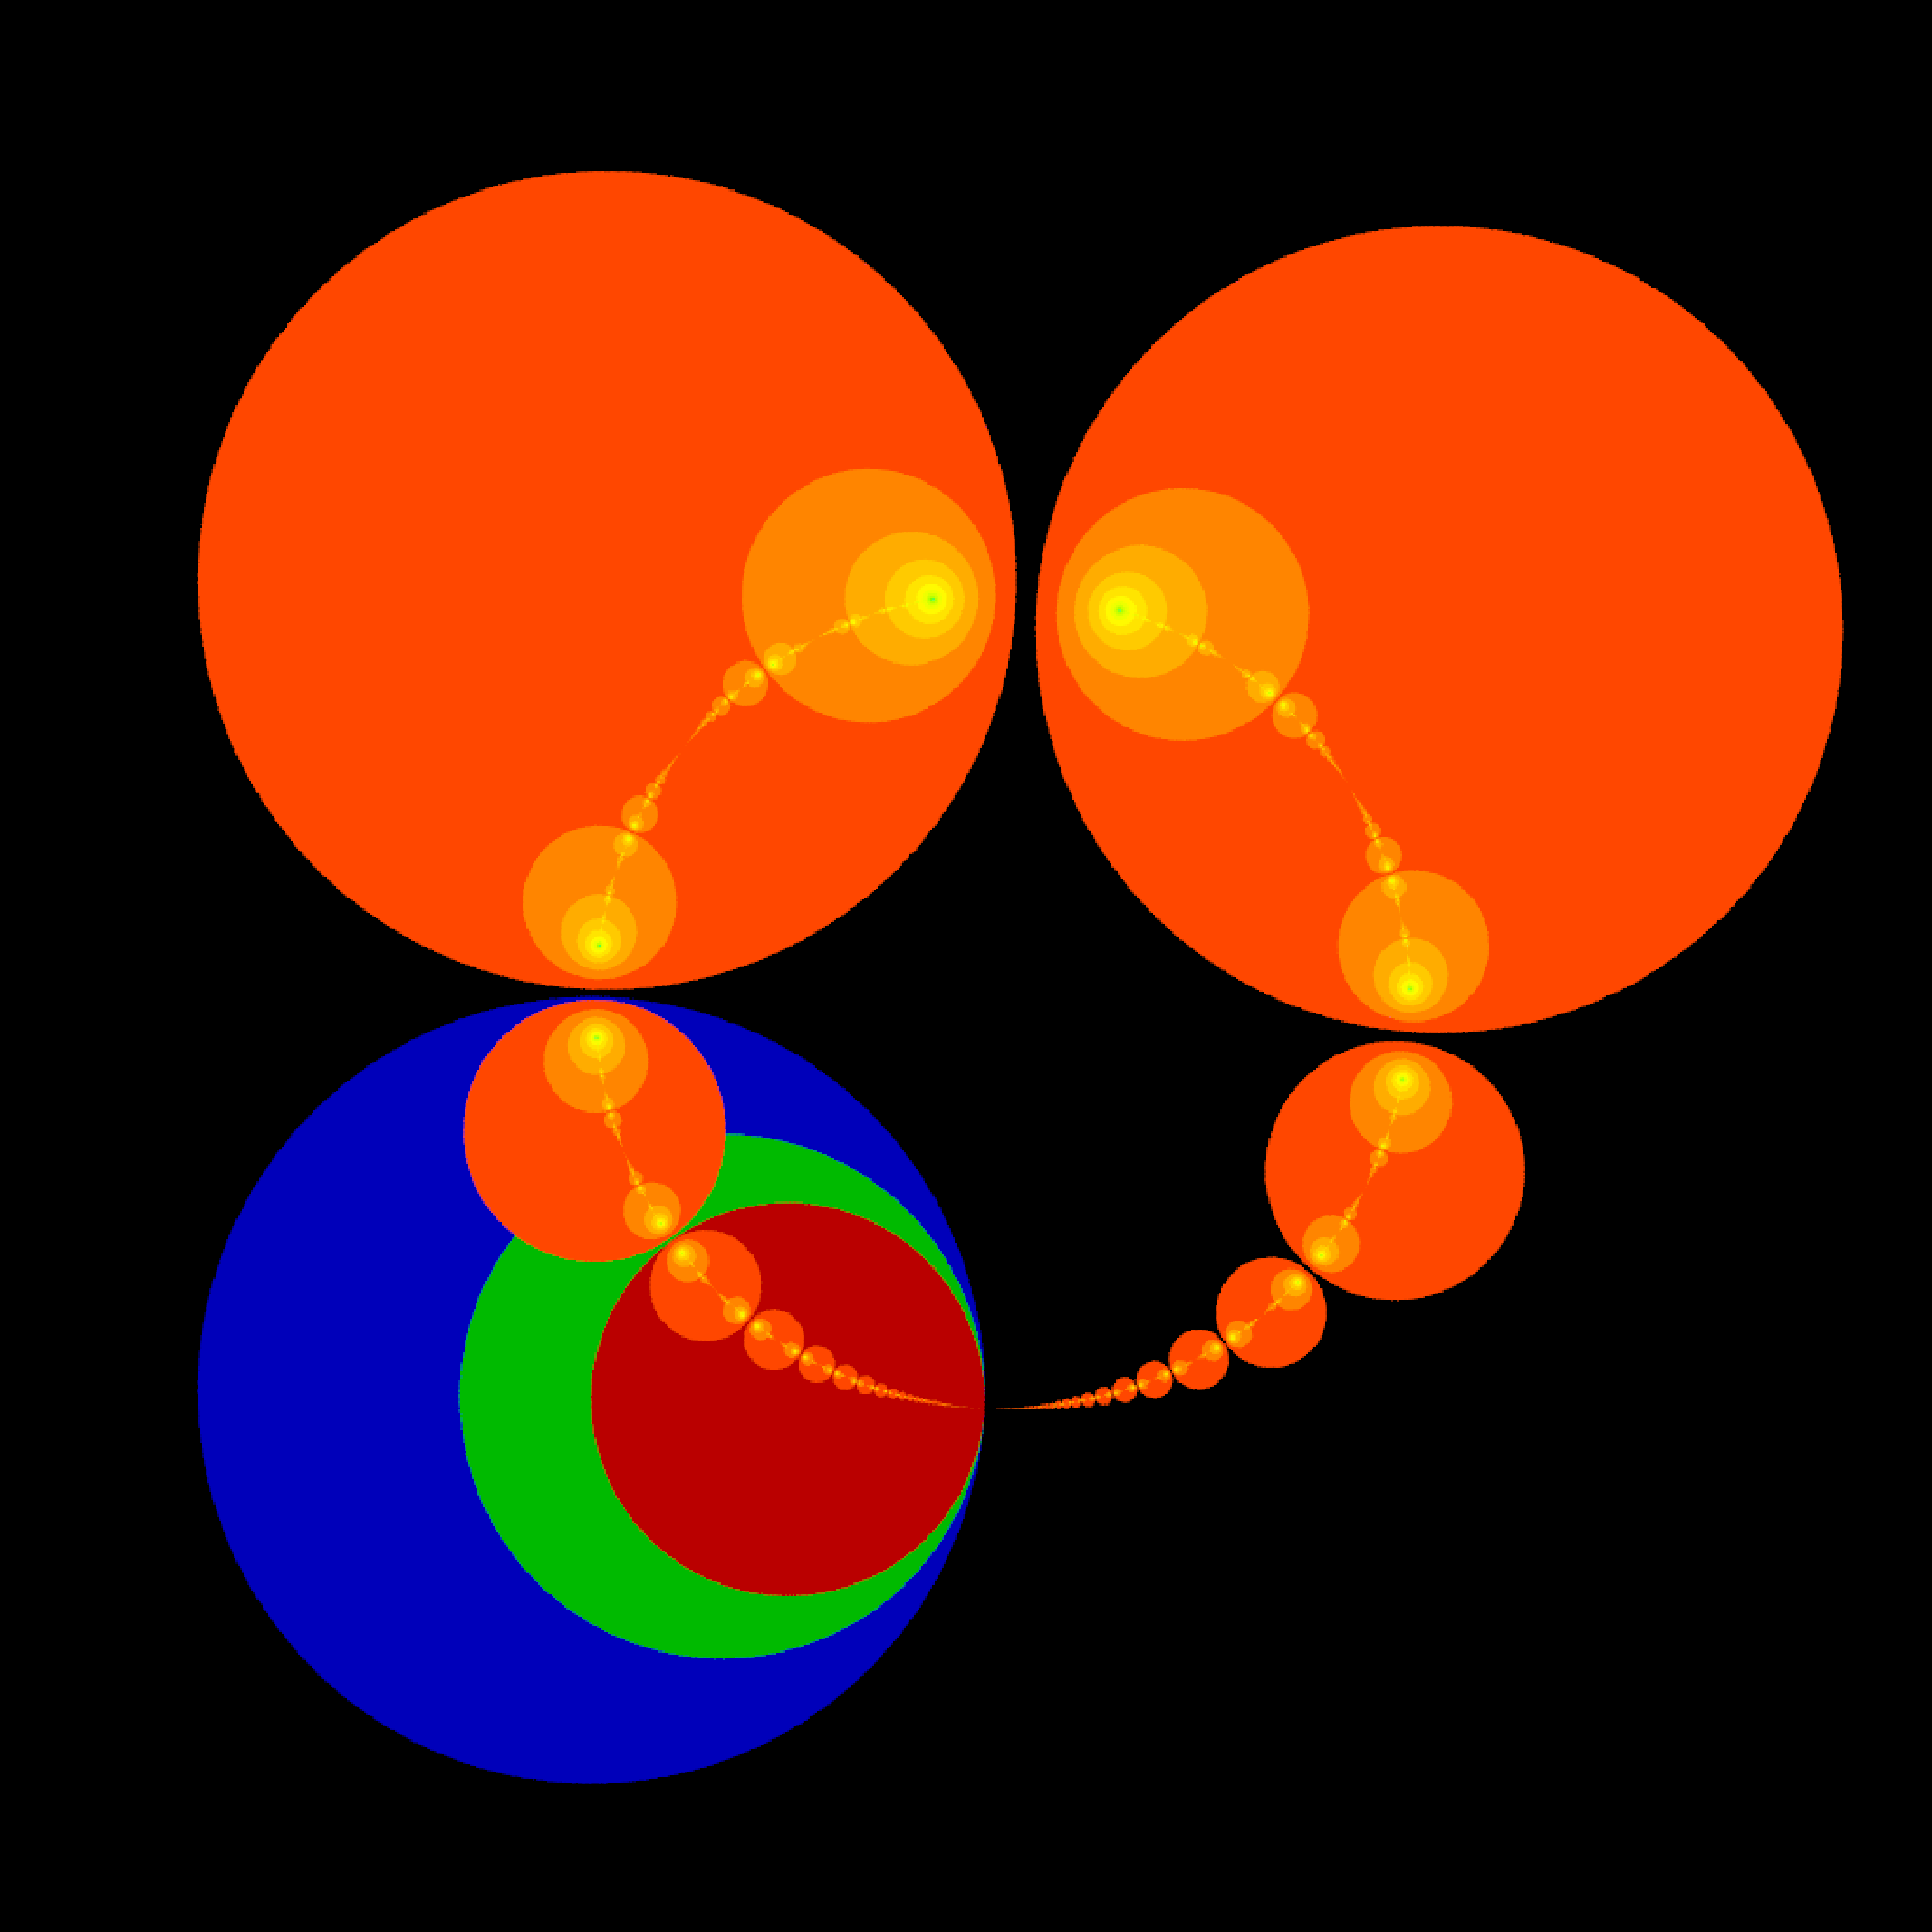
\includegraphics[ height=1.4in, keepaspectratio]{../src/img/application/2dGen/parabolicRect.pdf}
   \subcaption{\textit{Orbit}}
   \label{fig:parabolic2dOrb}
  \end{minipage}
  \hspace*{\fill}
  \caption{\textit{The orbit of Parabolic generator and \\a Schottky disk}}
  \label{fig:parabolic2d}
 \end{minipage}
\end{figure}

\begin{figure}[h!tbp]
  \begin{minipage}[t]{0.25\textwidth}
   \centering
   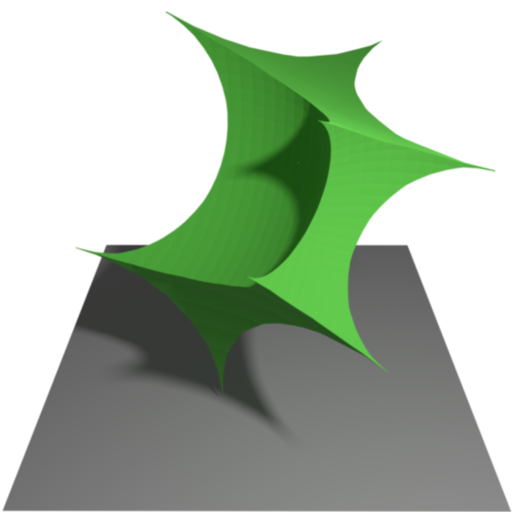
\includegraphics[height=1.2in,
   keepaspectratio]{../src/img/application/sphairahedron/cube.png}
   \caption{Cube-type sphairahedron.}
   \label{fig:cubeSphaira}
  \end{minipage}
  \hspace*{\fill}
 \begin{minipage}[t]{0.75\textwidth}
  \begin{minipage}[t]{0.25\textwidth}
   \centering
   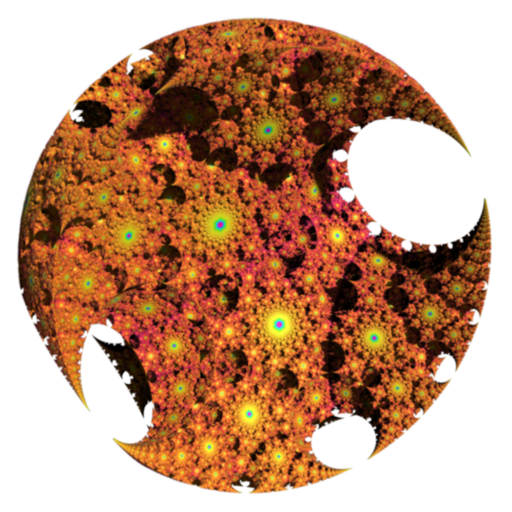
\includegraphics[height=1.2in,
   keepaspectratio]{../src/img/application/sphairahedron/quasi-sphere.png}
   \subcaption{}
  \end{minipage}
  \hspace*{\fill}
  \begin{minipage}[t]{0.25\textwidth}
   \centering
   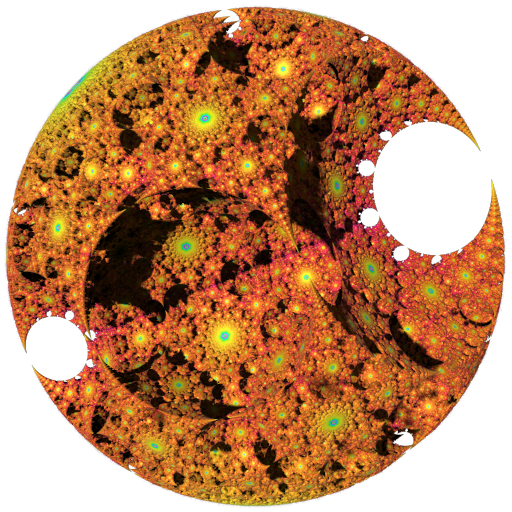
\includegraphics[height=1.2in,
   keepaspectratio]{../src/img/application/sphairahedron/other.png}
   \subcaption{}
  \end{minipage}
  \hspace*{\fill}
  \begin{minipage}[t]{0.25\textwidth}
   \centering
   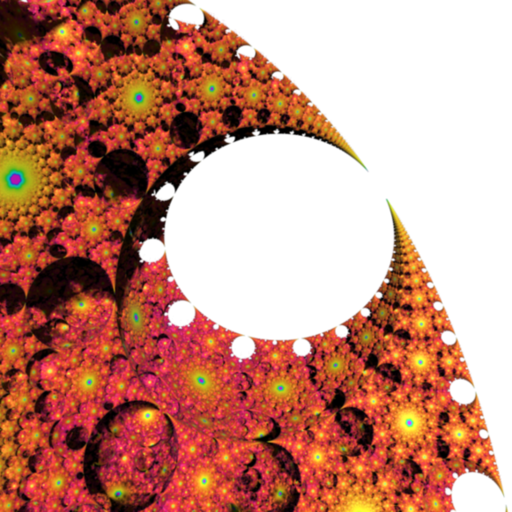
\includegraphics[height=1.2in,
   keepaspectratio]{../src/img/application/sphairahedron/quasi-sphereZoom.png}
   \subcaption{}
  \end{minipage}
  \hspace*{\fill}
  \caption{Images of a quasi-sphere rendered in different viewpoints.}
  \label{fig:quasi-sphere}
 \end{minipage}
\end{figure}

The third chapter introduces the visualization of Kleinian groups.
Chapter 3.1 shows a basic method of rendering Kleinian groups.
It has some defective to visualize Kleinian groups.
For example, see Figure \ref{fig:orbitCircles}; there are many nesting
disks. If we increase the number of initial disks, nesting disks also
increase exponential order.
To solve this problem, in chapter 3.2, we introduce the IIS.
IIS is applied to each point on the plane and computes nesting depth of
the disk which contains the point.
The process of the algorithm is as follows.
First of all, if the point is contained in one of the initial disks, we invert the
point in the boundary circle of the disk.
We continue applying inversions until the transformed point is in the
outside of all the initial disks.
IIS can be used in two and three-dimensional cases.
In chapter 3.3, we show some algorithms using IIS to draw three-dimensional
objects shown in Figure \ref{fig:3d}.

The fourth chapter gives some application.
We introduce four examples of the application of IIS.
First one shows how to render the interior or exterior of the
two-dimensional circle inversion fractals as in Figure \ref{fig:schottkyDivide}.
Secondly, we show the method to draw the edge of disks as shown in
Figure \ref{fig:circleEdge}.
Thirdly, the method to generate three or four-dimensional Kleinian groups with
a circle or sphere inversion. It enables us to tweak parameters of M\"obius
transformation intuitively.
See Figure \ref{fig:hyperbolic2d} and Figure \ref{fig:parabolic2d}.
The red, green, and blue regions represent M\"obius transformations and
apply them to an orange disk.
According to the configuration of regions, an orbit of the orange disks are
changed.
It can be extended to three-dimensional sphere inversion fractals.
Lastly, we can visualize sphairahedron fractals with IIS.
Sphairahedron is a polyhedron with spherical
faces as shown in Figure \ref{fig:cubeSphaira}.
Using inversions about their faces, we can make a tiling pattern
of the sphairahedron. See Figure \ref{fig:quasi-sphere}.
In many cases, the boundary of the tiling converges to a
three-dimensional fractal. 

Finally, the fifth chapter is the conclusion. We introduced an efficient algorithm
called IIS.
However, there are also Kleinian groups, which we cannot
visualize using IIS.
Our final goal is that for all Kleinian groups, we develop similar kind of
efficient algorithm as above and get mathematical results from obtained images.

\end{document}
